\section{Gestion des sections}

Voici les diff{\'e}rents sc{\'e}narios:\\

\section*{Enseignant}

\begin{center}
\scalebox{0.6}{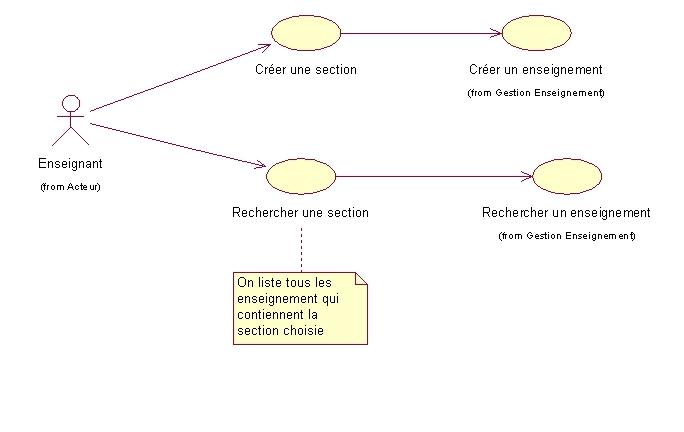
\includegraphics{images/Section_Enseigant.jpg}}\\
\end{center}

\begin{tabular}{|p{4cm}|c|p{4cm}|p{5cm}|}
\hline
  Fonction & Priorit{\'e} & Qualit{\'e} & Mesure \\
\hline
Cr�er une section & 4 & Fiable, Facile & Pas de redondance. Ergonomique.\\
\hline
Rechercher une section & 4 & Rapide et Complet & Permettre de lister rapidement les mati{\`e}res existantes et assurer le listing de toutes les mati{\`e}res sans en oublier.\\
\hline
\end{tabular}

\begin{center}
{\'e}chelle de mesure de la priorit{\'e}:

\scalebox{0.5}{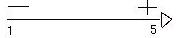
\includegraphics{images/echelle.jpg}}
\end{center}

\begin{itemize}
\item  {\bf Cr{\'e}er une section :}
	\begin{itemize}
	\item Pr{\'e}-requis : Etre log{\'e} 
	\item Description :Il s'identifie avec son login et son mot de passe. \\
	Il saisie la nouvelle section et valide.
	\item Post-requis : Une nouvelle section est cr{\'e}{\'e}e si elle n'existait pas.\\
	\end{itemize}

\item  {\bf Rechercher une section :}
	\begin{itemize}
	\item Pr{\'e}-requis : Etre log{\'e}.
	\item Description : Il s'identifie avec son login et son mot de passe.\\
	L'utilisateur demande le contenu d'une section.\\
	On liste tous les enseignements qui contiennent cette section.\\
	\end{itemize}
\end{itemize}

\section*{Administrateur}

\begin{center}
\scalebox{0.6}{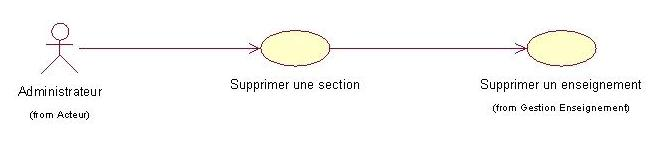
\includegraphics{images/Section_Administrateur.jpg}}\\
\end{center}

\begin{tabular}{|p{4cm}|c|p{4cm}|p{5cm}|}
\hline
  Fonction & Priorit{\'e} & Qualit{\'e} & Mesure \\
\hline
Supprimer une section & 4 & Fiable, Facile & On ne doit pas pouvoir effacer une section qui a encore des liens avec un enseignement.\\
\hline
\end{tabular}

\begin{center}
{\'e}chelle de mesure de la priorit{\'e}:

\scalebox{0.5}{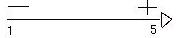
\includegraphics{images/echelle.jpg}}
\end{center}

\begin{itemize}
\item  {\bf Supprimer une section :}
	\begin{itemize}
	\item Pr{\'e}-requis : Etre log{\'e} 
	\item Description :Il s'identifie avec son login et son mot de passe. \\
	Il s�lectionne un section contenue dans aucun enseignement.\\
	Il clique l'option {\it Suppression} et valide son choix.
	\item Post-requis : La selection est supprim�e.
	\end{itemize}
\end{itemize}
